\documentclass{article}

% ICLR 2027 formatting had not been released when this skeleton was built.
% The verified ICLR 2026 template is deliberately not frozen as a future style.
\IfFileExists{iclr2027_conference.sty}{
  \usepackage{iclr2027_conference}
}{
  \usepackage[margin=1in]{geometry}
}
\usepackage{amsmath,amssymb,amsthm,booktabs,graphicx,hyperref,microtype}
\usepackage{xcolor}

\newtheorem{theorem}{Theorem}
\newtheorem{proposition}{Proposition}
\newcommand{\pending}{\textcolor{red}{\texttt{RESULT\_PENDING}}}
\newcommand{\tablepending}{\textcolor{red}{\texttt{TABLE\_PENDING\_RUNS}}}
\newcommand{\claimblocked}{\textcolor{red}{\texttt{CLAIM\_BLOCKED\_PENDING\_EVIDENCE}}}

\title{CoReGraph: Resource- and Budget-Aware Graph Expert Routing under
Compositional Deployment Shift}
\author{Anonymous Authors}

\begin{document}
\maketitle

\begin{abstract}
Graph models are deployed under contracts that jointly specify time, graph
visibility, construction, model selection, review budget, and compute
resources. A model or mixture selected under one contract can be inappropriate
when these coordinates change together, while the nominally strongest expert
may be unavailable at deployment. We formulate compositional deployment
generalisation for heterogeneous graph experts and introduce CoReGraph, a
router that encodes contract axes factorwise, combines label-free diagnostics,
masks infeasible experts, and optimises predictive utility together with
worst-contract regret, review budget, calibration, stability, and compute. We
prove a positive worst-contract regret lower bound for contract-independent
fixed mixtures when expert orderings cross, and give an axis-additive
compositional approximation bound with an explicit interaction residual.
Evaluation is pre-registered across temporal fraud tasks, controlled synthetic
shifts, and graph-OOD settings. Empirical results are \pending; no result claim
is made before the declared runs and paired analysis are complete.
\end{abstract}

\section{Introduction}

Graph-learning systems are usually compared under a single dataset split and a
single resource envelope. Deployment is less tidy. A detector may move from a
static graph to a rolling event stream, lose edge attributes, face a smaller
review budget, or run where a graph expert no longer fits in memory. These
changes are not merely covariate shift: they alter what is observable, what can
be selected, and which actions are feasible.

Prior graph-OOD benchmarks make distribution shifts explicit
\cite{gui2022good}, while graph mixtures route among computation paths or
feature/structure experts \cite{wang2023gmoe,zeng2024mowst}. GraphMETRO aligns
experts for mixtures of shift components \cite{wu2024graphmetro}. These works
motivate a sharper deployment question: can a router generalise to an unseen
\emph{combination} of known contract coordinates while respecting review and
compute constraints?

We study that question through four contributions:

\begin{enumerate}
  \item a six-axis compositional deployment-contract problem with separate
  node, edge, and transaction prediction units;
  \item CoReGraph, a resource- and budget-aware expert router using factorised
  contract encoding, label-free diagnostics, feasibility masks, fallback,
  abstention, and routing-stability regularisation;
  \item exact lower-bound and compositional-error results with machine-checked
  numerical examples; and
  \item ContractShiftBench, a pre-registered evaluation across fraud,
  graph-OOD, and controlled synthetic surfaces.
\end{enumerate}

FraudShiftBench is prior evaluation infrastructure, not the method contribution
of this paper. The present manuscript does not reuse its completed result
tables as evidence for CoReGraph.

\section{Related work}

\paragraph{Graph OOD generalisation.}
GOOD provides explicit covariate and concept-shift environments for node and
graph prediction \cite{gui2022good}. CIGA learns causally invariant subgraphs
\cite{chen2022ciga}; EERM explores graph edits to extrapolate across node
environments \cite{wu2022eerm}; and GraphMETRO uses aligned experts and a gate
to model composed graph shifts \cite{wu2024graphmetro}. CoReGraph differs in
treating observability, construction, selection, review budget, and resource
availability as typed deployment coordinates, and in evaluating held-out
combinations with a feasible-expert oracle.

\paragraph{Graph mixtures and routing.}
GMoE routes nodes among message-passing experts \cite{wang2023gmoe}. Mowst
combines a weak feature expert with a strong graph expert through confidence
\cite{zeng2024mowst}. Concurrent STEM-GNN uses tokenised experts and stability
regularisation under graph corruptions \cite{guo2026stem}. CoReGraph instead
routes among heterogeneous pretrained expert families and conditions on a
factorised deployment contract. This distinction must be tested empirically
against the strongest compatible implementations; novelty is not inferred from
architecture prose alone.

\paragraph{Temporal graphs and adaptation.}
TGN represents dynamic graphs as timed event streams with memory
\cite{rossi2020tgn}. The event-stream baseline in this work uses official TGN
code where task semantics permit; a snapshot approximation is diagnostic only.
Unlabelled target adaptation is reported separately from domain
generalisation and few-label adaptation.

\paragraph{Robust, selective, and resource-aware learning.}
Group DRO targets worst-group risk \cite{sagawa2020groupdro}; VREx penalises
environment-risk variance \cite{krueger2021vrex}. Selective prediction permits
abstention when risk is high \cite{geifman2017selective}. CoReGraph combines
these ideas at the contract level with explicit feasible-expert masks and
review-budget outcomes. Oracle experts are offline evaluation ceilings, not
deployment procedures.

\section{Problem formulation}

A deployment contract is
$c=(c^{\mathrm{time}},c^{\mathrm{vis}},c^{\mathrm{build}},
c^{\mathrm{select}},c^{\mathrm{budget}},c^{\mathrm{resource}})$.
Each coordinate is typed. It determines an admissible graph view
$G_c$, a prediction unit, target-access regime, feasible expert set
$\mathcal A(c)$, and operational metric. Source contracts
$\mathcal C_s$ are labelled for training. A target contract
$c_t\notin\mathcal C_s$ may combine axis values observed separately in
$\mathcal C_s$.

Let expert $e$ emit a score $s_e(x;G_c)$ and incur a declared offline risk
$R_c(e)$. A router emits weights
$w_\theta(x,c,d)\in\Delta^{|\mathcal A(c)|}$ from the contract and label-free
diagnostics $d$. Infeasible experts are masked before normalisation. The routed
score is
\[
  s_\theta(x,c)=\sum_{e\in\mathcal A(c)}w_{\theta,e}(x,c,d)s_e(x;G_c).
\]
For V5 target evaluation, the primary offline oracle chooses the lower Brier
loss among each row's feasible expert predictions and the same frozen-cost
abstention action available to the method. The primary
\texttt{contract\_regret\_vs\_feasible\_row\_oracle} averages method loss minus
that matched-action row-oracle loss. A best fixed feasible non-abstaining expert
over the whole contract is retained only as a separately named diagnostic. No
oracle is queried at deployment.
The older contract-level feasible oracle and instance-clairvoyant oracle remain
source-training or theory terminology only; neither defines the V5 primary
target metric.

We distinguish domain generalisation with no target access,
unlabelled target adaptation, and few-label target adaptation. Thresholds,
target priors, and diagnostics inherit this access type. Node, edge, and
transaction outcomes are never pooled as independent rows in one leaderboard.
Target contract metadata and an operational target capacity may be known at
inference; target labels are not available for fitting, threshold selection,
or routing.

The optimisation surrogate is binary cross-entropy and is reported, when
needed, as BCE-surrogate contract regret. Selective risk is the zero--one
error on accepted predictions. These quantities have different losses and are
not compared numerically under a shared generic regret label.

\section{CoReGraph}

\begin{figure}[t]
  \centering
  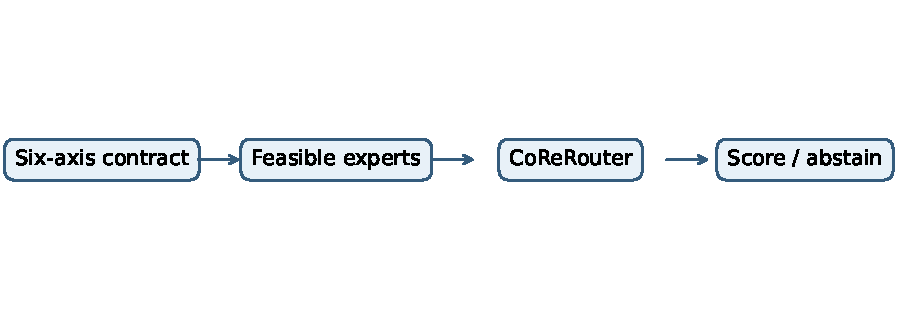
\includegraphics[width=\linewidth]{figures/figure_1_system_schematic.pdf}
  \caption{CoReGraph execution path. This is a system schematic, not an
  empirical result. Feasibility is imposed before routing, and no-feasible-
  expert cases abstain.}
  \label{fig:system}
\end{figure}

\paragraph{Factorised contract encoder.}
Each categorical coordinate has an embedding with an unknown token. Continuous
budget, memory, latency, and window values are concatenated after scaling.
Optional pairwise dot-product interactions capture low-order composition.
Axis dropout and bounded contract noise prevent brittle dependence on complete
metadata. An atomic contract-ID encoder and a no-contract encoder serve as
baselines; the atomic encoder maps held-out IDs to an unknown token.

\paragraph{Label-free diagnostics.}
The router can consume expert scores, confidence, entropy, score and rank
disagreement, visible degree and isolation, missingness, temporal instability,
graph density, unlabelled score drift, predicted prevalence, cost, and
availability. Every diagnostic declares its graph view, granularity, target
access, and label requirement. Label-dependent graph-harm diagnostics are
source-only and cannot enter target inference.

\paragraph{Masked routing and safe behaviour.}
CoReRouter scores expert tokens using a linear, MLP, or small attention router.
Unavailable experts receive negative-infinite routing logits and exactly zero
weight. If no expert is feasible, the system abstains. Otherwise it can fall
back to a feature-only expert, the fixed source-validation winner, a static
average, or a top-two mixture. Outputs include weights, selected expert,
abstention probability, entropy, expected compute, and an explanation record.

\paragraph{Objective.}
For source contract groups, the configurable loss is
\[
 \mathcal L =
 \lambda_{\mathrm{avg}}\mathcal L_{\mathrm{pred}}+
 \lambda_{\mathrm{reg}}\operatorname{CVaR}_\alpha(\mathrm{Reg}_c)+
 \lambda_{\mathrm{bud}}\mathcal L_{\mathrm{budget}}+
 \lambda_{\mathrm{stab}}\mathcal L_{\mathrm{stability}}+
 \lambda_{\mathrm{cost}}\mathcal L_{\mathrm{compute}}+
 \lambda_{\mathrm{cal}}\mathcal L_{\mathrm{calibration}}.
\]
The budget term is a smooth top-$K$ surrogate; we do not claim exact
optimisation of discontinuous Recall@$K$. Stability covers contract
perturbations, score noise, and availability masks.

\begin{figure}[t]
  \centering
  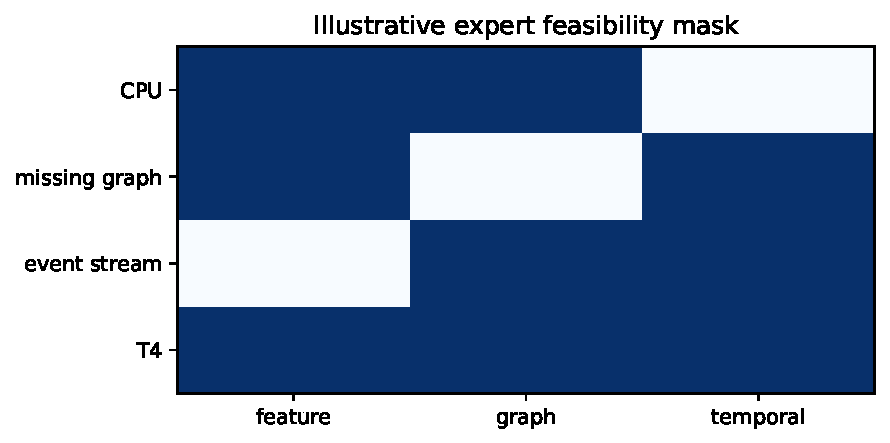
\includegraphics[width=.72\linewidth]{figures/figure_3_resource_mask.pdf}
  \caption{Illustrative feasibility masks under four resource/visibility
  settings. Shading is schematic and contains no measured availability.}
  \label{fig:resource-mask}
\end{figure}

\section{Theory}

\begin{figure}[t]
  \centering
  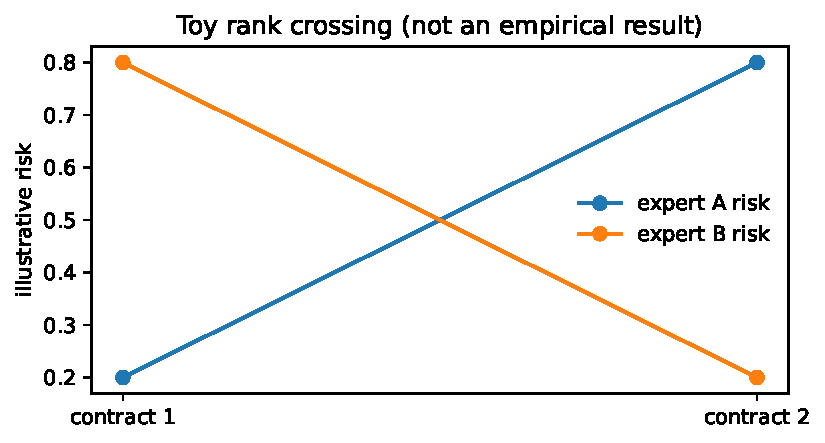
\includegraphics[width=.70\linewidth]{figures/figure_2_fixed_mixture_counterexample.pdf}
  \caption{Toy crossing-risk construction used to illustrate the
  fixed-mixture lower bound. Values are synthetic and not experiment results.}
  \label{fig:crossing}
\end{figure}

\begin{theorem}[Fixed-mixture regret; \texttt{PROVED}]
Consider two experts and two contracts. On contract one their risks are
$(0,\delta_1)$ and on contract two they are $(\delta_2,0)$, where
$\delta_1,\delta_2>0$. A contract-independent randomised mixture that selects
expert one with probability $w$ has worst-contract regret at least
\[
  \frac{\delta_1\delta_2}{\delta_1+\delta_2}>0.
\]
The bound is tight, while a contract-aware selector has zero regret.
\end{theorem}

\begin{proof}
The mixture regrets are $(1-w)\delta_1$ and $w\delta_2$. Their maximum is
minimised when they are equal, since decreasing either side of the intersection
increases the other maximum. Solving
$(1-w)\delta_1=w\delta_2$ gives
$w^\star=\delta_1/(\delta_1+\delta_2)$ and the stated value. A
contract-aware selector chooses expert one on contract one and expert two on
contract two.
\end{proof}

\paragraph{Failure of the premise.}
If either gap is zero, or one expert is optimal on both contracts, the positive
lower bound need not hold.

\begin{theorem}[Axis-additive approximation; \texttt{PROVED}]
Let the risk of a candidate routing action $a$ under a $d$-axis contract
$c=(c_1,\ldots,c_d)$ decompose as
\[
 R(a,c)=b(a)+\sum_{j=1}^d f_j(a,c_j)+h(a,c),
\]
where $|h(a,c)|\leq\epsilon_{\mathrm{int}}$. Suppose estimates satisfy
$|\widehat f_j(a,c_j)-f_j(a,c_j)|\leq\epsilon_j$ for every axis value present
in source contracts, and the learned router's optimisation error relative to
the minimiser of the estimated additive risk is at most
$\epsilon_{\mathrm{router}}$. For an unseen combination containing only those
observed axis values, its excess true risk over the best action is at most
\[
 2\sum_{j=1}^d\epsilon_j+
 2\epsilon_{\mathrm{int}}+\epsilon_{\mathrm{router}}.
\]
\end{theorem}

\begin{proof}
For any action, the difference between true risk and estimated additive risk is
at most $\sum_j\epsilon_j+\epsilon_{\mathrm{int}}$ by the triangle
inequality. Apply this bound once to the learned action and once to the true
optimal action, and insert the assumed optimisation error between their
estimated risks.
\end{proof}

\paragraph{Interpretation and counterexample.}
The guarantee does not cover an unseen axis value. It becomes vacuous when the
interaction residual is large. An XOR interaction between two contract axes
has zero marginal axis effects but nonzero joint risk, providing a direct
counterexample to factorisation without the residual term.


Both results are labelled \texttt{PROVED} in the proof audit. They concern
randomised expert selection risk and an axis-additive approximation class,
respectively; they do not establish real-world fraud performance. The appendix
states failure cases and numerical checks.

\section{Experimental design}

\paragraph{Surfaces.}
Fraud tasks comprise Elliptic and DGraphFin node prediction, Elliptic++ as a
correlated temporal corroboration, and IBM AML Small/Medium transaction-edge
prediction. T-Finance is included only if source, licence, and genuine
timestamps pass audit. General graph OOD uses three task-compatible GOOD node
settings. Controlled synthetic regimes vary feature and graph signal,
homophily, direction, drift, missing inputs, resource masks, and review budget.

\paragraph{Splits and access.}
Primary evaluation holds out unseen combinations of observed axis values.
Leave-one-axis-value, resource, budget, construction, visibility, temporal, and
random-environment splits are secondary controls. Domain generalisation,
unlabelled TTA, and few-label access are separate families.

\paragraph{Baselines and ablations.}
Baselines include individual feature/graph/tree/temporal experts, simple
averaging, source-validation selection, Mowst, GraphMETRO when licensed,
task-compatible graph OOD, official TGN, Group DRO, VREx, GraphSafe, atomic
contract routing, no-contract routing, and the offline feasible oracle. Pending
or unlicensed official code is excluded rather than approximated under its
name. Ablations remove contract axes, interactions, diagnostics, regret, CVaR,
budget, compute, stability, fallback, or abstention.

\paragraph{Outcomes and inference.}
Primary outcomes are AUPRC, Recall@0.5\%, Recall@1\%, Recall@2\%,
budget-curve area, mean, maximum, and CVaR regret, selective risk, and compute.
Inference pairs exact dataset--task--target-contract--fold contexts, averages
contexts within seed, and treats the seed as the inferential block. Exact
Wilcoxon, paired permutation, and seed-block bootstrap analyses replace normal
approximations. Holm families are frozen before any final-run outcomes are
inspected. Worst-contract comparisons use paired target-contract outcomes or
contract regret rather than minima of unpaired raw scores.

\section{Results}

\tablepending

No experiment number is populated in this skeleton. The following claims are
blocked until their typed evidence predicates, prediction exports, seed
coverage, exact target-contract cells, paired analysis, effect thresholds,
confidence intervals, and Holm family pass:

\begin{itemize}
  \item \claimblocked: CoReGraph improves worst-contract AUPRC.
  \item \claimblocked: CoReGraph reduces maximum or CVaR regret.
  \item \claimblocked: gains hold on both real fraud datasets.
  \item \claimblocked: factorised encoding generalises to unseen combinations.
  \item \claimblocked: resource-aware routing improves compute-normalised utility.
\end{itemize}

Figures 4--6 and every empirical table are generated only from validated result
manifests after the final ten-seed campaign. V5 primary regret uses the
row-wise feasible expert-or-abstain hindsight oracle; the best fixed feasible
non-abstaining expert remains a separate diagnostic.

\section{Limitations}

Contracts simplify organisational and data-collection processes into six
coordinates; omitted interactions may dominate. Label-free diagnostics can
still shift or be strategically manipulated. The feasible oracle depends on
which experts were implemented and measured, and is not a population optimum.
Fraud datasets differ in task unit, provenance, label mechanism, and timestamp
quality, so they are not pooled as independent replications. Elliptic++ is
correlated with Elliptic. IBM AML is synthetic. DGraphFin and T-Finance have
provider/licence boundaries. Review-budget costs are application-dependent.

Official baseline coverage may remain incomplete when upstream licences or
task adapters are unavailable. Synthetic mechanisms demonstrate identifiability
and failure modes, not fraud realism. Fixed-dataset seed inference quantifies
algorithmic variability and does not justify claims about an unspecified
population of datasets.

\section{Conclusion}

CoReGraph treats graph deployment as a compositional contract rather than a
single split label. Its implementation makes graph visibility, target access,
expert feasibility, budget, compute, fallback, abstention, and evidence scope
machine-checkable. The method and evaluation are ready for the declared runs;
empirical conclusions remain \pending.


\paragraph{Reproducibility statement.}
The appendix and anonymous artifact will specify the six-axis deployment
contract, graph-view construction, task adapters, official-baseline pins,
configuration hashes, saved predictions, telemetry, and the frozen analysis
plan. Provider data and credentials will not be redistributed.

\paragraph{Ethics statement.}
Fraud detection is a high-impact decision-support setting. We report ranking,
review-budget, calibration, abstention, and resource outcomes without treating
model predictions as adjudications. Dataset licences, privacy boundaries,
false-positive burdens, and human review capacity are explicit deployment
coordinates. No personally identifying provider data is included in the
artifact.

\bibliographystyle{plain}
\bibliography{references}

\appendix
\section{Contract schema and leakage guarantees}
The artifact provides the canonical JSON schema, exclusion rules, fold-specific
train/validation/target graph views, and leakage sentinels.

\section{Task and dataset cards}
Node, edge, and transaction identifiers, label mappings, timestamp quality,
dataset licences, and acquisition checksums are reported separately.

\section{Complete proofs}
The proof-status audit and numerical scripts are part of the anonymous artifact.

\section{Full experiment and analysis manifests}
All smoke, screening, final, ablation, GOOD, fraud, resource, and theory rows
are generated before execution. Final prediction and result hashes will be
listed here after evidence import.

\section{LLM usage disclosure placeholder}
\texttt{POLICY\_CHECK\_AT\_SUBMISSION}. The currently available ICLR 2026
author guide requires disclosure of significant LLM use. The policy for the
actual target year must be checked from the official author guide.


\end{document}
